\documentclass{article}

\usepackage{listings}
\usepackage[pdftex]{graphicx}
\title{Python exercises 1}
\begin{document}
\maketitle
\section{Simple arithmetic}
\begin{enumerate}
\item 3/5 + 2
\item 3/float(5) + 2
\item 3./5 + 2
\item 3/5 + 2.
\item 3**2
\item 3**(2+5)
\item (3**2)+5
\item 3./5/2
\item 3/5/2.
\item 3/5./2
\end{enumerate}

\section{Program flow}
\begin{enumerate}
\item Make a 'for' loop that sums '1' hundred times.
\item Make a 'for' loop that sums the numbers from 1 to 100. Change the code to sum only the odd numbers.
\item Make a variable word1='gateman'. Make a for loop that inverts the letter order of word1.
\item Write the codes that produce the depicted program flows:\\
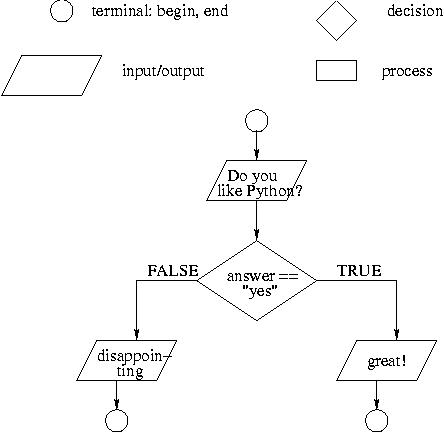
\includegraphics[scale=0.5]{./p21.jpg}

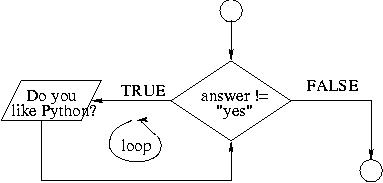
\includegraphics[scale=0.5]{./p22.jpg}
\end{enumerate}
\pagebreak
\section{Script}
Create a .py file with the following content and make sure you understand every line. Execute it.

\begin{lstlisting}
#!/usr/bin/env python
#
# A program for numbers
#

a = 3 - 4 + 10
b = 5 * 6
c = 7.0/8.0
print "Hello World, these are the values:", a, b, c
print "Increment", a, "by one: "
a = a +1
print a
print "The sum of", a, "and", b, "is?"
a = ' are'
b = "you"
c = "years old. Don't you think?"
d = b + a
number = input("Input a number ")
print d, number, c
\end{lstlisting}

\section{Lists}
Please open the file list1.py and follow the instructions.
After you are done, there is also list2.py.
\end{document}